\documentclass[12pt,a4paper]{article}
\usepackage{graphicx}
\usepackage{amsmath}
\usepackage{bm}
\usepackage{interval}
\begin{document}
\section*{Problem 10}
We can observe that the distribution of the update times of the weight $\bm{w}$ is concentrated around 100.
Most of them are in the interval $\interval{95}{105}$, which is about $\frac{N}{2}$.
By the figure 1, we can find out that the update times is about half of the numbers of the data.
\begin{figure}[hbp]
    \centering
    \begin{minipage}{0.48\linewidth}
        \centering
        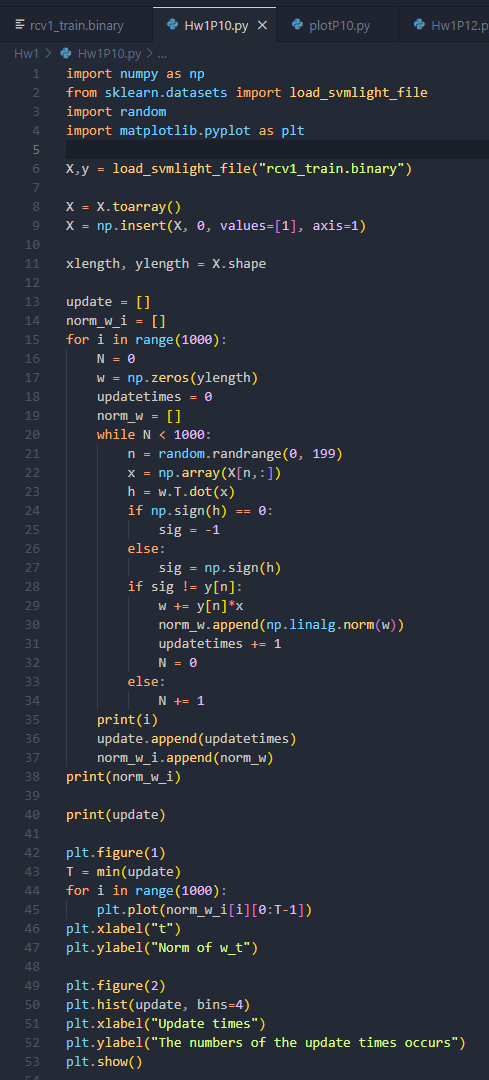
\includegraphics[width = \linewidth]{Hw1P10 snapshot.png}
        \caption{snapshot}
    \end{minipage}\hfil
    \begin{minipage}{0.48\linewidth}
        \centering
        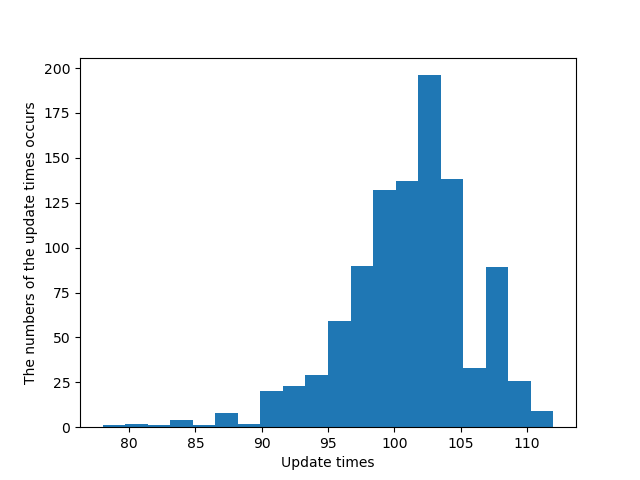
\includegraphics[width = \linewidth]{Hw1P10.png}
        \caption{historgram}
    \end{minipage}\hfil
\end{figure}
\newpage
\section*{Problem 11}    

\begin{figure}[hbp]
    \centering
    \begin{minipage}{0.48\linewidth}
        \centering
        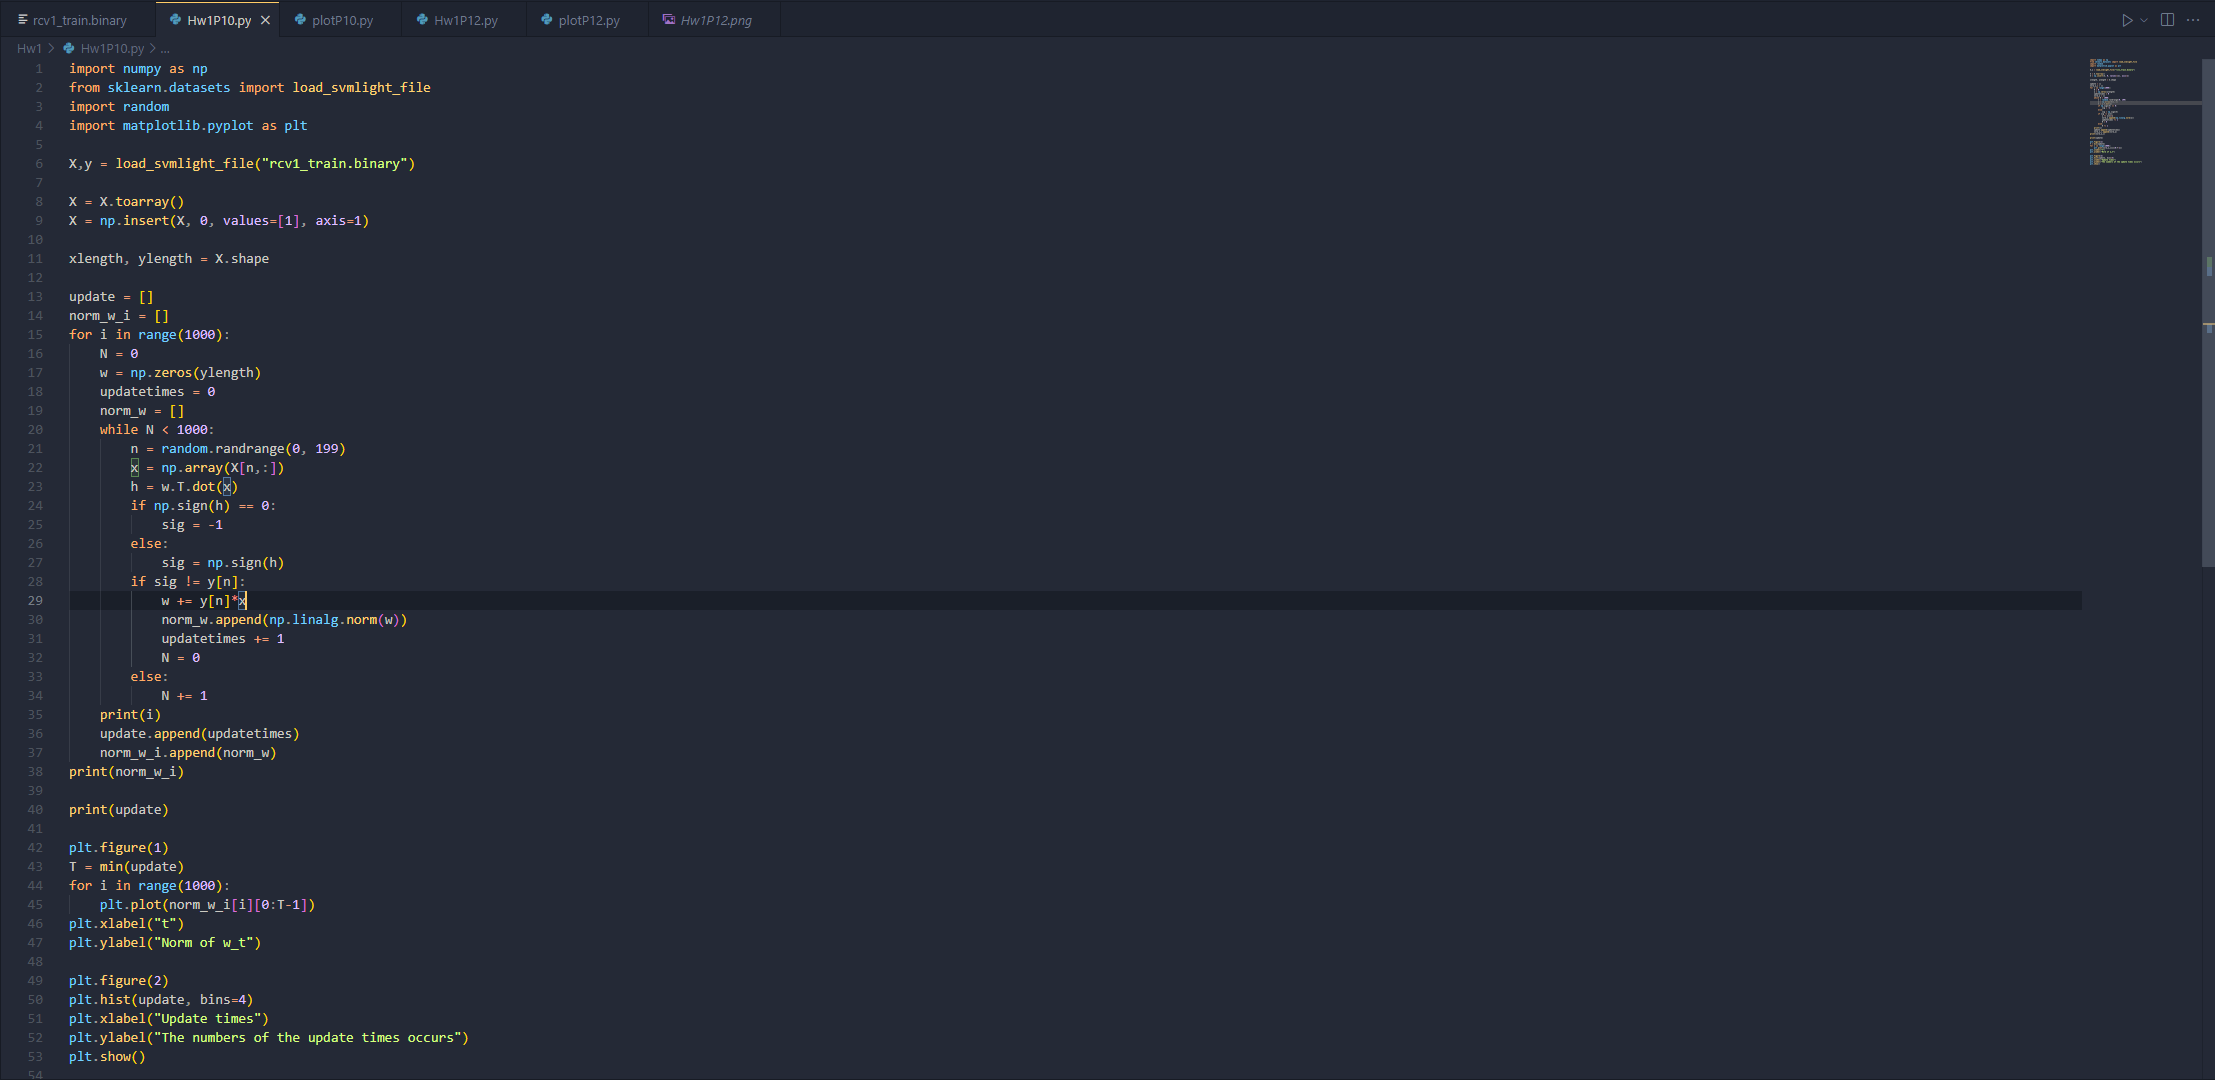
\includegraphics[width = \linewidth]{Hw1P11 snapshot.png}
        \caption{snapshot}
    \end{minipage}\hfil
    \begin{minipage}{0.48\linewidth}
        \centering
        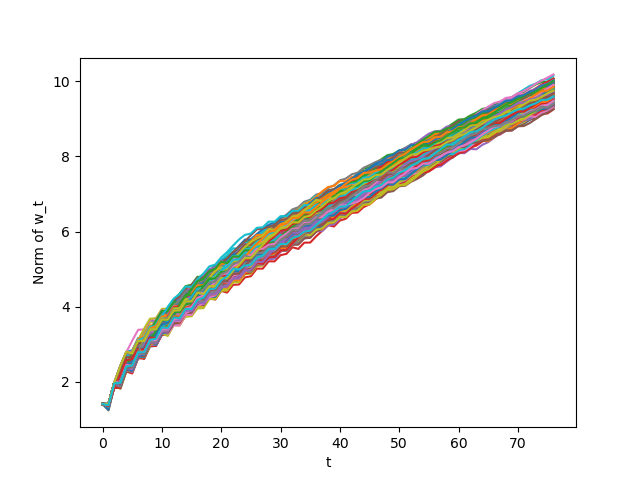
\includegraphics[width = \linewidth]{Hw1P11.png}
        \caption{plot}
    \end{minipage}\hfil
\end{figure}

\newpage
\section*{Problem 12}    
For the P12, we update $n(t)$ only when $\bm{w}_{t}$ does not change. 
Compare with Figure 2 we can observe that most of the update times are still in $\interval{95}{105}$.
But it looks more concentrated then the histogram in P10. That is, the update times are more stable than P10.   
\begin{figure}[hbp]
    \centering
    \begin{minipage}{0.48\linewidth}
        \centering
        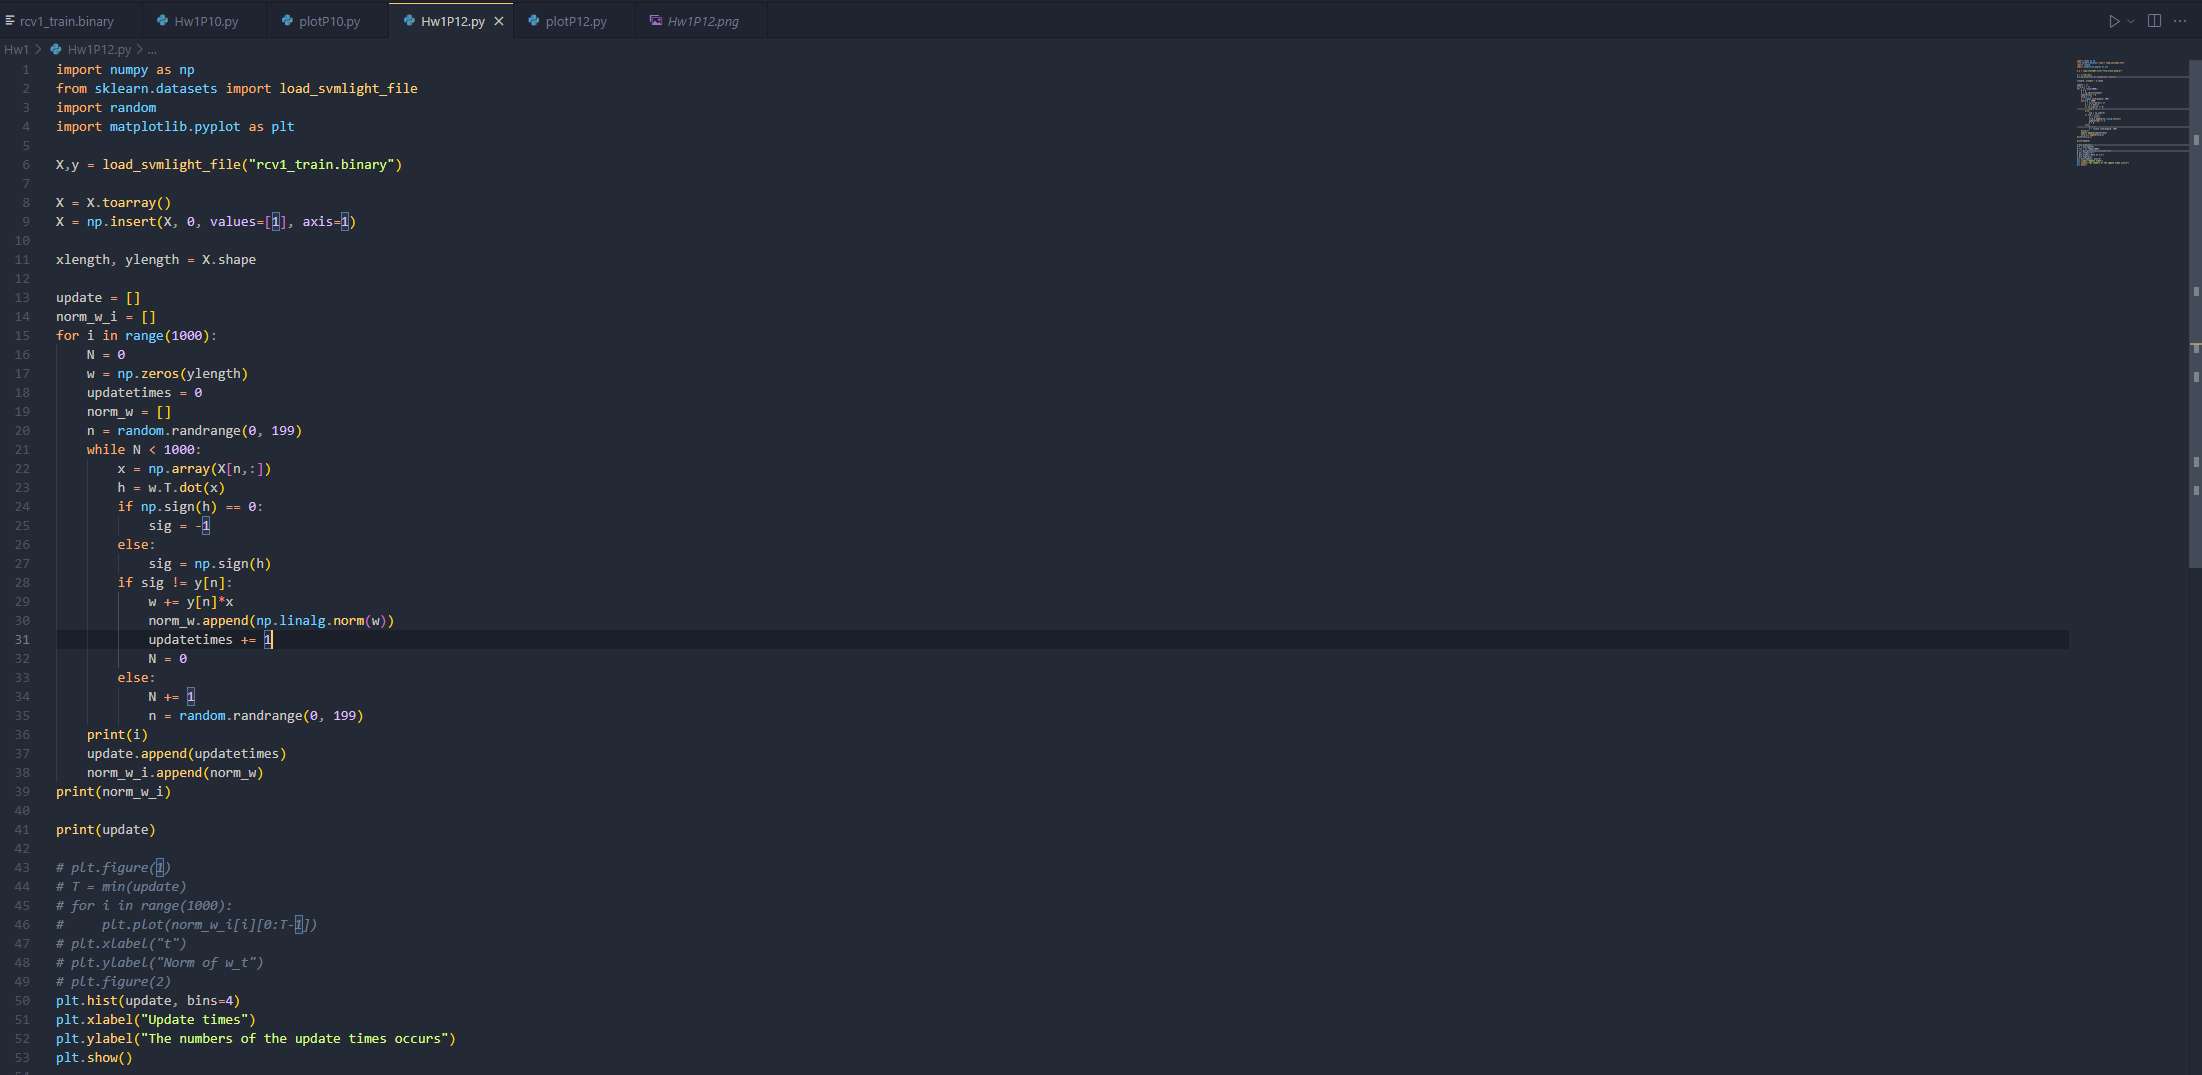
\includegraphics[width = \linewidth]{Hw1P12 snapshot.png}
        \caption{snapshot}
    \end{minipage}\hfil
    \begin{minipage}{0.48\linewidth}
        \centering
        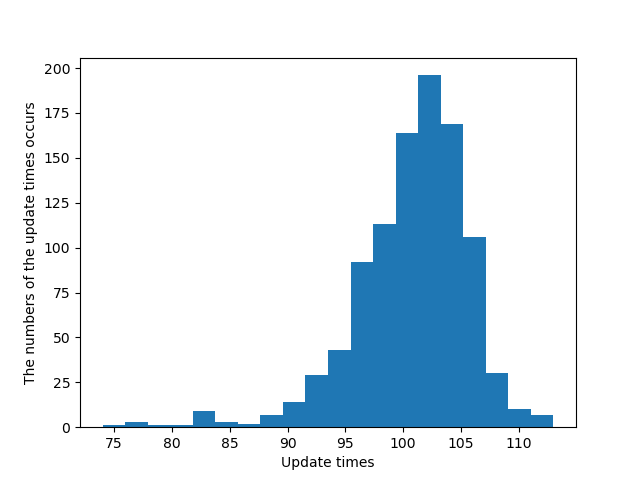
\includegraphics[width = \linewidth]{Hw1P12.png}
        \caption{historgram}
    \end{minipage}\hfil
\end{figure}
\end{document}
